\documentclass{llncs}
\usepackage[T1]{fontenc}
\usepackage{graphicx}
\usepackage{enumitem}
\usepackage{amsmath}
\usepackage{listings}
\usepackage{tikz}
\usepackage{epstopdf}
\usepackage{multirow}
\usepackage{todonotes}

\title{Evaluating the Effectiveness of AEX-Notify against SGX Single-Stepping Attackers}
\author{Wicked Wench}
\institute{	University of L\"ubeck, Germany}
% TODO: For the camera-ready submission
%\author{Basil Ugbomoiko\inst{1} \quad Daniel Knaack\inst{1}}
%\institute{	University of L\"ubeck, Germany\\
%	\email{\{basil.ugbomoiko,daniel.knaack\}@student.uni-luebeck.de}}

\begin{document}

\maketitle

\begin{abstract}
  Trusted execution environments (TEEs) like Intel's Software Guard Extensions (SGX)
  offer a promising avenue for securing applications by executing them within secure enclaves.
  However, recent advancements in side-channel attack techniques, such as SGX-Step,
  pose significant threats to the security guarantees provided by SGX.
  SGX-Step uses the APIC timer to precisely interrupt the enclave after each instruction,
  effectively stepping through the execution one instruction at a time.
  These single-stepping capabilities allow much greater granularity for side-channel,
  thereby enhancing the feasibility of side-channel attacks.
  In response to this threat, AEX-Notify has been proposed as a potential mitigation against SGX-Step.
  AEX-Notify is both a hardware extension and a software mitigation that tries
  to prevent adversaries from single-stepping enclaves.
  This paper analyzes the security of AEX-Notify and evaluates its
  effectiveness against deterministic single-stepping.
\end{abstract}

\section{Motivation}

Modern computing relies heavily on privileged system software to manage interactions and ensure security.
However, traditional operating system kernels are susceptible to bugs and vulnerabilities
due to their large codebase written in unsafe languages.
To address this, recent research has focused on Protected Module Architectures (PMAs),
aiming to support isolated execution of security-sensitive components
called enclaves with minimal Trusted Computing Base (TCB).
Intel’s Software Guard eXtensions (SGX) \cite{Intel16,Intel17} represent a significant advancement,
providing hardware-enforced trusted computing guarantees.
However, vulnerabilities have emerged, particularly in information leakage
through attacks exploiting various system components.
These vulnerabilities undermine the security promises of SGX.

SGX-Step presents a novel framework to address SGX vulnerabilities by enabling
precise monitoring of enclave execution at the instruction level.
Unlike previous methods, SGX-Step achieves true single-stepping for any enclave program,
significantly enhancing the resolution of existing attacks.
The framework comprises a Linux kernel driver and a runtime library,
providing the means to interrupt enclave execution at the instruction level
for detailed observation and analysis.

\paragraph{Introduction to AEX-Notify}
\begin{itemize}
  \item Overview of AEX-Notify
  \item Potential benefits of using AEX-Notify
\end{itemize}

\paragraph{Research Question and Objectives}
\begin{itemize}
  \item Formulation of the \textbf{research question}:
    Is it possible to gather control-flow information of victim programs running
    in SGX enclaves when the victim protects the execution of the enclave with
    AEX-Notify?
  \item \textbf{Project goals}:
    Our goal is to evaluate the effectiveness of AEX-Notify against SGX-step by
    constructing an example program where the SGX-Step attack works and testing
    this program once with AEX-Notify enabled and once without. We will compare
    the results to see how much information we can gain about control-flow
    information with and without AEX-Notify enabled.
\end{itemize}

\section{Background}

This section provides a comprehensive review of existing research and frameworks
relevant to the evaluation of AEX-Notify against SGX single-stepping attackers.
In particular, we outline the workings of Intel SGX and
discuss how SGX-Step leverages the APIC timer to single-step enclaves.
Following this, we examine CopyCat, which leverages SGX-Step to extract
control-flow information from enclaves, highlighting potential security
vulnerabilities.
Finally, we look into the details of AEX-Notify and
how it prevents the single-stepping capabilities of SGX-Step.

\subsection{Intel SGX}

Intel Software Guard Extensions (SGX) is a security feature introduced by Intel
that enables the creation of secure enclaves within applications \cite{CostanD16}.
Enclaves provide a protected execution environment for sensitive code and data,
ensuring confidentiality and integrity even if the host system is compromised.
Key components of SGX include:

\begin{itemize}
  \item \textbf{Memory Management:}
    SGX enforces memory isolation between enclaves and non-enclave code,
    preventing unauthorized access to enclave data.
  \item \textbf{Interrupt/Exception Handling:}
    When an interrupt occurs, it triggers an AEX (Asynchronous Enclave eXit),
    which saves the application state in the current SSA.
    However, the enclave application has no mechanism (without AEX-Notify) to detect an interrupt.
  \item \textbf{TCS, SSA, TCS.CSSA:}
    SGX defines structures such as Thread Control Structure (TCS) and Saved State Area (SSA)
    to manage enclave execution and state transitions.
    \texttt{TCS.CSSA} refers to the current saved state area within the TCS.
  \item \textbf{EENTER, EEXIT:}
    SGX instructions for entering and exiting enclaves,
    facilitating the secure transition of control flow between enclave and non-enclave code.
  \item \textbf{Security Goals:}
    It's important to note that the primary goal of SGX is to protect
    the confidentiality and integrity of enclave data and code,
    rather than providing defenses against side-channel attacks,
    which are the responsibility of enclave developers \cite{CostanD16}.
\end{itemize}

\subsection{SGX-Step}

SGX-Step is a framework designed to address vulnerabilities in SGX
by enabling precise monitoring of enclave execution at the instruction level \cite{ArnautovTGKMPLM16}.
It utilizes the APIC timer to interrupt enclave execution at specific intervals,
allowing for detailed observation and analysis.
Previous methods for interrupting enclave execution often resulted in large time jitter,
making it difficult to precisely control the timing of interrupts.
SGX-Step overcomes these challenges by configuring the APIC timer in user space,
enabling finer control over interrupt timing and reducing time jitter \cite{ArnautovTGKMPLM16}.

\todo[inline]{Explain why SGX-Step is important $\to$ It enables side-channel attacks at instruction-level granularity}

\subsection{CopyCat}

CopyCat \cite{MoghimiBHPS20} utilizes the framework
to infer fine-grained control-flow information from SGX enclaves.
It improves upon traditional page-fault adversaries,
that can only page accesses at a 4 KiB resolution,
with the single-stepping capabilities of SGX-Step.

\begin{figure}[t]
  \centering
  \includegraphics{square-and-multiply.pdf}
  \caption{\textbf{TODO}: Add caption.}
  \label{fig:square-and-multiply}
\end{figure}

In a typical square-and-multiply implementation,
we can use page faults to extract the key.
On each iteration we can induce a fault by clearing the execute permission on
the page with the \emph{square} function.
Tracking access in each iteration, we can fully recover the key from only page faults.

Traditional page-fault adversaries fail at recovering the key when the entire
square-and-multiply procedure fits on a single page.
CopyCat overcomes this challenge by single-stepping the enclave and counting the
number of instructions until a data page was accessed.
In the example of square-and-multiply, there are two data accesses of interest.
The first is the access to the cipher text that is squared on each iteration.
The second is the write to the output whenever the key bit is one.
By counting the number of instructions between each data access,
CopyCat can recover the key even if the cipher text, output and key are on the same page.

\todo[inline]{Add paragraph explaining why this is a problem in the context of
  the SGX attacker model. Because technically side-channel attacks are not a
  concern for SGX, but they still implemented AEX-Notify.}

\subsection{AEX-Notify}
\label{sec:aex-notify}

\begin{figure}[t]
  \centering
  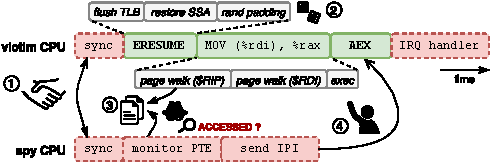
\includegraphics{images/sgx-step-pte.pdf}
  \caption{\todo[inline]{Add a proper caption here.}}
  \label{fig:sgx-step-pte}
\end{figure}

To counter SGX-Step and the attack vectors that it enables, AEX-Notify has been proposed.
The purpose of AEX-Notify is to stop attackers from reliably single-stepping an enclave,
which mitigates many attacks based on SGX-Step like CopyCat.

Constable et al. \cite{ConstableBCXXAK23} list the root cause behind the effectiveness of SGX-Step as the assisted page-table walk.
Before resuming the enclave, the SGX-Step attack clears the accessed bit on the pages,
which causes a page fault when executing the first instruction.
This induces additional latency in the execution of the instruction, because
the processor has to walk the page table again.
Thus, there is a large time frame where the interrupt of the timer could
arrive and land exactly on the first instruction.
The goal of AEX-Notify is to reduce the latency of the first instruction
and make it impossible to reliably land on the first instruction.

The first part of AEX-Notify is the hardware extension.
It introduces a new flag in the SSA frame, called \texttt{AEXNOTIFY}.
By enabling this flag, we can change the behavior of the \texttt{ERESUME} instruction,
which resumes the enclave.
Usually, \texttt{ERESUME} restores the previous process context,
however, when the \texttt{AEXNOTIFY} bit is enabled,
a custom exception handler is executed.
The exception handler is responsible for handling the AEX and
can resume the enclave application with an additional instruction, called \texttt{EDECCSSA}.
This instruction decrements \texttt{TCS.CSSA} and restores the context of the enclave application.

The second part of AEX-Notify is the custom exception handler.
The goal of the exception handler is to reduce the latency of the first instruction.
In order to achieve this, it is important that the first instruction never causes any page faults.
Otherwise, we would need to walk the page table again which would increase the latency of the first instruction.
Thus, the software mitigation implements a prefetcher.
This prefetcher will always fetch necessary code and data pages of the resumed
instruction which ensures that no faults can occur.

With the software mitigation enabled, an interrupt can arrive at three possible
locations during the execution.
First, it could arrive too early and land in our prefetching code.
This would not cause any problems as resuming the enclave a second time would
call the prefetcher again and would load the same pages as before.
Next, the interrupt could arrive to late and land after the first instruction.
In this case, we would have executed more than one instruction which means
that we have successfully avoided single-stepping.
Last, it could arrive perfectly on the first instruction.
This is the exact case that we are trying to avoid.
However, since the code and data pages for this instruction have already been prefetched,
it is unlikely that an interrupt would arrive exactly on the first instruction.

\todo[inline]{
  Explain more details about the software part, i.e. the constant-time decoder,
  c3 cache, etc. This could also be something in the work description.
}

\section{Work Description}

The goal of this project is to analyze the effectiveness of AEX-Notify.

\subsection{Initializing SGX-Step}

SGX-Step requires careful configuration of the APIC timer
since it is crucial for the attack to work.
If the value is too small, then we will zero-step and execute the same instruction multiple times.
If the value is too large, then we will multi-step and execute multiple instruction.
We have used an example application provided in the SGX-Step repository for this purpose.
This example consists only of a series of \texttt{nop} instructions and
reports the instruction pointer after each interrupt using the \texttt{EDBRD}.
If the instruction pointer is incremented by one instruction each interrupt,
then we can be sure that we are single-stepping the enclave.

Usually the reported addresses are enough to configure the timer
since each address is incremented by one when the timer is configured correctly.
Thus, we know that the timer is configured incorrectly if the addresses stay
the same or vary too much.
The problem with AEX-Notify is that interrupting the enclave not only
interrupts the enclave but also the exception handler.
Thus, the application will also report addresses from the exception handler.
We have written a simple tool that uses the debug information from the binary and
automatically translates these addresses to their source code location in the trusted runtime system.

\subsection{Single-stepping Attack Implementation}

The single-stepping attack, also known as the Zigzagger attack,
aims to exploit vulnerabilities in SGX enclaves
by interrupting enclave execution at precise intervals.
This section provides a detailed overview of the Zigzagger attack methods and a step-by-step implementation guide.

\textbf{Introduction to Zigzagger Attack Methods:}
The Zigzagger attack utilizes techniques to interrupt SGX enclave execution at the instruction level,
thereby enabling the extraction of control-flow information.
It involves precise timing to resume execution either before or after specific instructions,
allowing an attacker to gather sensitive information.

\textbf{Step-by-step Implementation Guide:}
\begin{enumerate}
  \item \textbf{Identifying Target Enclaves:} The first step involves selecting target SGX enclaves susceptible to single-stepping attacks.
  \item \textbf{Setting Interrupt Intervals:} Determine the optimal timing intervals for interrupting enclave execution to capture control-flow information effectively.
  \item \textbf{Implementing Interruption Mechanism:} Develop the mechanism to interrupt enclave execution using techniques such as APIC timers.
  \item \textbf{Fine-tuning Timing:} Adjust timing parameters to ensure the interruption occurs at critical points during enclave execution.
  \item \textbf{Testing and Validation:} Validate the implementation by running test scenarios to verify the effectiveness of the single-stepping attack in extracting control-flow information.
\end{enumerate}

\subsection{Experimental Setup}

This section outlines the hardware and software specifications of the experimental environment, including configuration details necessary for conducting the evaluation.

\textbf{Hardware and Software Specifications:}
\begin{itemize}
  \item Intel Core i7 10th Gen, 16GB DDR4 RAM, and SSD storage.
  \item Ubuntu 20.04 LTS (Linux kernel version 5.10) with SGX driver support. Use SGX SDK for enclave development.
\end{itemize}

\textbf{Configuration Details:}
\begin{itemize}
  \item
    Configure SGX environment with appropriate BIOS settings and SGX driver installation.
    Utilize SGX SDK for enclave development.
  \item
    Set up the environment to execute the single-stepping attack.
    Select target enclaves and configure attack parameters for testing.
\end{itemize}

\subsection{Implementation Details for Applying AEX-Notify}

Explain how AEX-Notify is integrated into the experimental setup

\textbf{Integration with Experimental Setup:}
\begin{itemize}
  \item
    Integrate AEX-Notify into existing SGX environment
    by modifying enclave code to enable AEX-Notify functionality.
    Ensure compatibility with enclave execution flow and security requirements.
\end{itemize}

\textbf{Configuration and Setup Details:}
\begin{itemize}
  \item Enable AEX-Notify within the SGX enclave environment
    by setting appropriate flags or parameters during enclave initialization.
    Configure AEX-Notify to intercept and handle exceptions caused by single-stepping attacks.
\end{itemize}

We enable AEX-Notify by adding an additional field in the enclave configuration.
The exception handler is preconfigured to use the trusted runtime system of the SDK.
This is the same handler as described in Section~\ref{sec:aex-notify}.

\section{Results}

As the most basic requirement,
we were no longer able to single-step the enclave after enabling AEX-Notify.
Using a page-fault, we could always reliably interrupt the application
before executing the first instruction of the target code.
However, it was not possible to reliably execute one or even multiple instructions after the first.

The application reports the instruction pointer of the enclave
and after reporting the first instruction of our target code correctly,
we could only see addresses that were in the exception handler.
This means that each interrupt always arrives too soon and
lands in the exception handler instead of the enclave itself.

\begin{itemize}
  \item After enabling AEX-Notify, we can no longer single-step (This is the most basic requirement, so not really special)
  \item The interrupt lands in the exception handler most of the time
  \item For pages without any return, the interrupt arrives during the C3 cache lookup.
  \item Where does the exception handler rollback when interrupting the small assembly stub?
    It goes back to the original exception handler, i.e. the first stage and not the second stage.
  \item \textbf{TODO}: Can we differentiate between zero-step and multi-step by simulating a cache attack?
\end{itemize}

\section{Conclusion and Future Work}
\begin{itemize}
    \item Summary of key findings
    \item Potential enhancements to AEX-Notify
    \item Future research directions
\end{itemize}

\bibliographystyle{alpha}
%\bibliographystyle{splncs03}
\bibliography{references}
\end{document}
